% =============================================================================
% COPYRIGHT AND DISCLAIMER
% =============================================================================
% This file is provided as a convenience template for competition participants.
% By using it, you accept full responsibility for compliance with all applicable
% copyright, licensing, and usage rules of the Association for Computing
% Machinery (ACM) and of any LaTeX packages you load (including, without
% limitation, the "acmart" document class and related ACM materials).
%
% Consult ACM's official publication, template, and copyright policies before
% using this setup for any purpose other than this competition. Do not assume
% that this template may be reused, redistributed, or submitted elsewhere
% without independently verifying ACM's current rules.
%
% Use of the "acmart" class, the "sigconf" option, or ACM-style formatting in
% this template does NOT mean that this report, this competition, its organizers,
% or any resulting PDF is sponsored, endorsed, affiliated with, or published by
% ACM. ACM trademarks and branding remain the property of ACM.
%
% Template packages live in preamble.tex.
% Citations live in main.bib. Edit this file with your paper content.
% =============================================================================

\documentclass[sigconf]{acmart}
% =============================================================================
% Template setup — participants normally do not edit this file.
% Author content belongs in main.tex; citations belong in main.bib.
% \documentclass lives in main.tex so Overleaf does not treat this file as root.
% =============================================================================

% --- Competition / non-ACM-submission friendly rights metadata -------------
\setcopyright{none}
\settopmatter{printacmref=false}
\acmConference[Kaggle Competition]{Filament Segmentation Challenge}{2026}{\href{https://www.kaggle.com/competitions/filament-segmentation-2026}{kaggle.com/competitions/filament-segmentation-2026}}
\acmBooktitle{Competition Report}
\acmDOI{}
\acmISBN{}

% --- Author guidance text --------------------------------------------------
% \guide{...} is gray italic while \guideStyletrue; omitted from the PDF if false.
% Flip the switch in main.tex after % =============================================================================
% Template setup — participants normally do not edit this file.
% Author content belongs in main.tex; citations belong in main.bib.
% \documentclass lives in main.tex so Overleaf does not treat this file as root.
% =============================================================================

% --- Competition / non-ACM-submission friendly rights metadata -------------
\setcopyright{none}
\settopmatter{printacmref=false}
\acmConference[Kaggle Competition]{Filament Segmentation Challenge}{2026}{\href{https://www.kaggle.com/competitions/filament-segmentation-2026}{kaggle.com/competitions/filament-segmentation-2026}}
\acmBooktitle{Competition Report}
\acmDOI{}
\acmISBN{}

% --- Author guidance text --------------------------------------------------
% \guide{...} is gray italic while \guideStyletrue; omitted from the PDF if false.
% Flip the switch in main.tex after % =============================================================================
% Template setup — participants normally do not edit this file.
% Author content belongs in main.tex; citations belong in main.bib.
% \documentclass lives in main.tex so Overleaf does not treat this file as root.
% =============================================================================

% --- Competition / non-ACM-submission friendly rights metadata -------------
\setcopyright{none}
\settopmatter{printacmref=false}
\acmConference[Kaggle Competition]{Filament Segmentation Challenge}{2026}{\href{https://www.kaggle.com/competitions/filament-segmentation-2026}{kaggle.com/competitions/filament-segmentation-2026}}
\acmBooktitle{Competition Report}
\acmDOI{}
\acmISBN{}

% --- Author guidance text --------------------------------------------------
% \guide{...} is gray italic while \guideStyletrue; omitted from the PDF if false.
% Flip the switch in main.tex after \input{preamble}.
%
% Do not use \guide{...} for \email{...}.
\usepackage{xcolor}
\newif\ifguideStyle
\guideStyletrue
\newcommand{\guide}[1]{%
  \ifguideStyle
    {\color{gray!65}\itshape #1}%
  \fi
}

% --- Math ------------------------------------------------------------------
% Do NOT load amssymb (or amsfonts): acmart already loads newtxmath, which
% defines the same symbols (e.g. \Bbbk) and causes a conflict on Overleaf.
% amsmath is already provided by acmart; mathtools extends it.
\usepackage{mathtools}

% --- Figures ---------------------------------------------------------------
% graphicx is already loaded by acmart
\usepackage{subcaption}

% --- Tables ----------------------------------------------------------------
% booktabs is already loaded by acmart
\usepackage{tabularx}
\usepackage{multirow}

% --- Bibliography style is set in main.tex (ACM-Reference-Format) ----------
.
%
% Do not use \guide{...} for \email{...}.
\usepackage{xcolor}
\newif\ifguideStyle
\guideStyletrue
\newcommand{\guide}[1]{%
  \ifguideStyle
    {\color{gray!65}\itshape #1}%
  \fi
}

% --- Math ------------------------------------------------------------------
% Do NOT load amssymb (or amsfonts): acmart already loads newtxmath, which
% defines the same symbols (e.g. \Bbbk) and causes a conflict on Overleaf.
% amsmath is already provided by acmart; mathtools extends it.
\usepackage{mathtools}

% --- Figures ---------------------------------------------------------------
% graphicx is already loaded by acmart
\usepackage{subcaption}

% --- Tables ----------------------------------------------------------------
% booktabs is already loaded by acmart
\usepackage{tabularx}
\usepackage{multirow}

% --- Bibliography style is set in main.tex (ACM-Reference-Format) ----------
.
%
% Do not use \guide{...} for \email{...}.
\usepackage{xcolor}
\newif\ifguideStyle
\guideStyletrue
\newcommand{\guide}[1]{%
  \ifguideStyle
    {\color{gray!65}\itshape #1}%
  \fi
}

% --- Math ------------------------------------------------------------------
% Do NOT load amssymb (or amsfonts): acmart already loads newtxmath, which
% defines the same symbols (e.g. \Bbbk) and causes a conflict on Overleaf.
% amsmath is already provided by acmart; mathtools extends it.
\usepackage{mathtools}

% --- Figures ---------------------------------------------------------------
% graphicx is already loaded by acmart
\usepackage{subcaption}

% --- Tables ----------------------------------------------------------------
% booktabs is already loaded by acmart
\usepackage{tabularx}
\usepackage{multirow}

% --- Bibliography style is set in main.tex (ACM-Reference-Format) ----------


% Guide styling: \guideStyletrue = show gray italic hints; \guideStylefalse = omit them
\guideStylefalse

\begin{document}
\setlength{\abovedisplayskip}{4.2pt plus 1pt minus 1pt}
\setlength{\belowdisplayskip}{4.2pt plus 1pt minus 1pt}
\setlength{\textfloatsep}{8pt plus 2pt minus 2pt}
\setlength{\dbltextfloatsep}{8pt plus 2pt minus 2pt}

\title[Topology-Preserving Cooperative Filament Segmentation]{Preserving Thin Topology Under Multi-Observer Disagreement: Physics-Guided Cooperative Segmentation of Solar Filaments}
\subtitle{A Solution to the Solar Filament Segmentation Challenge 2026} % DO NOT CHANGE

\author{Samiul Islam}
\affiliation{%
  \institution{Islamic University of Technology}
  \city{Dhaka}
  \country{Bangladesh}
}
\email{samiulislam@iut-dhaka.edu}

\begin{abstract}
    This report describes our solution to the Solar Filament Segmentation Challenge~2026, a Kaggle competition on automatic segmentation of solar filaments in GONG H-$\alpha$ observations. Standard panoptic architectures stall near $0.33$ Panoptic Quality (PQ) on MAGFiLO. Before scaling network capacity, we ran mask-perturbation and inter-observer experiments across $6{,}982$ ground-truth instances to isolate the mathematical bottlenecks. Downsampling ground-truth masks onto a $512 \times 512$ grid forfeits $0.0801$ PQ before any prediction error. Eroding contours by $2$~px wipes out $96.6\%$ of thin ribbons ($\le 6$~px) below $\text{IoU} > 0.50$, while pairwise human agreement reaches only $0.3367$ PQ. Guided by these bounds, we introduce a four-stage full-resolution framework. Huber IRLS limb regression slices an unblurred $1888 \times 1888$ five-channel chromospheric tensor that cuts cross-observatory variance $\eta^2$ by $37\%$ and triples contrast SNR to $4.77$. An ignore-shielded $1408^2$ Mask R-CNN with seven aspect ratios ($0.15$--$6.5$) proposes object boxes. A decoupled cooperative network pairs an ImageNet-22k ConvNeXt-Small context stream with a full-resolution anisotropic strip U-Net via $\tanh(\alpha)$ cross-scale bridges and asymmetric co-teaching on inverse-$\sqrt{\text{area}}$ Signed Distance Field (SDF) consensus targets. Geodesic hysteresis, dual-detector Voronoi saddle cuts, waist bridges, and a $24$-feature solar-rotation expected-PQ scorer assemble disjoint masks, reaching $0.4523$ three-fold out-of-fold PQ ($0.5363$ on $\ge 2$-vote consensus) and $0.40$ on the Kaggle Public Leaderboard.
\end{abstract}

\maketitle

% ==================================== %
%              INTRODUCTION            %
% ==================================== %
\section{Introduction}
    This report goes over the details of our submitted solution to the Solar Filament Segmentation Challenge~2026 \cite{filament-segmentation-2026}. The challenge, launched on July~10,~2026, is organized by the Earth-Space AI Research (ESAIR) Lab\footnote{\href{https://www.esairlab.com/home}{www.esairlab.com/}}. This challenge utilizes the MAGFiLO dataset for evaluation of the segmentation algorithms \cite{ahmadzadeh2024dataset}.

    Off-the-shelf panoptic models fail hard here. A scratch ResUNet-34 baseline reached $0.3332$ PQ on Fold~0, emitting $1{,}022$ false positives and fracturing $135$ ribbons into $351$ fragments. Experiments across $707$ training disks ($1{,}154$ observer entries and $8{,}199$ masks across six GONG stations, 2011--2022) and $180$ test disks traced that collapse to three coupled pathologies: resizing and wide Gaussian blur erase $1$--$3$~px lateral barbs, watershed cuts shatter branched Y-junctions, and raw multi-observer supervision mixes dilated contours with unverified single-annotator fibrils.

\begin{figure*}[t]
    \centering
    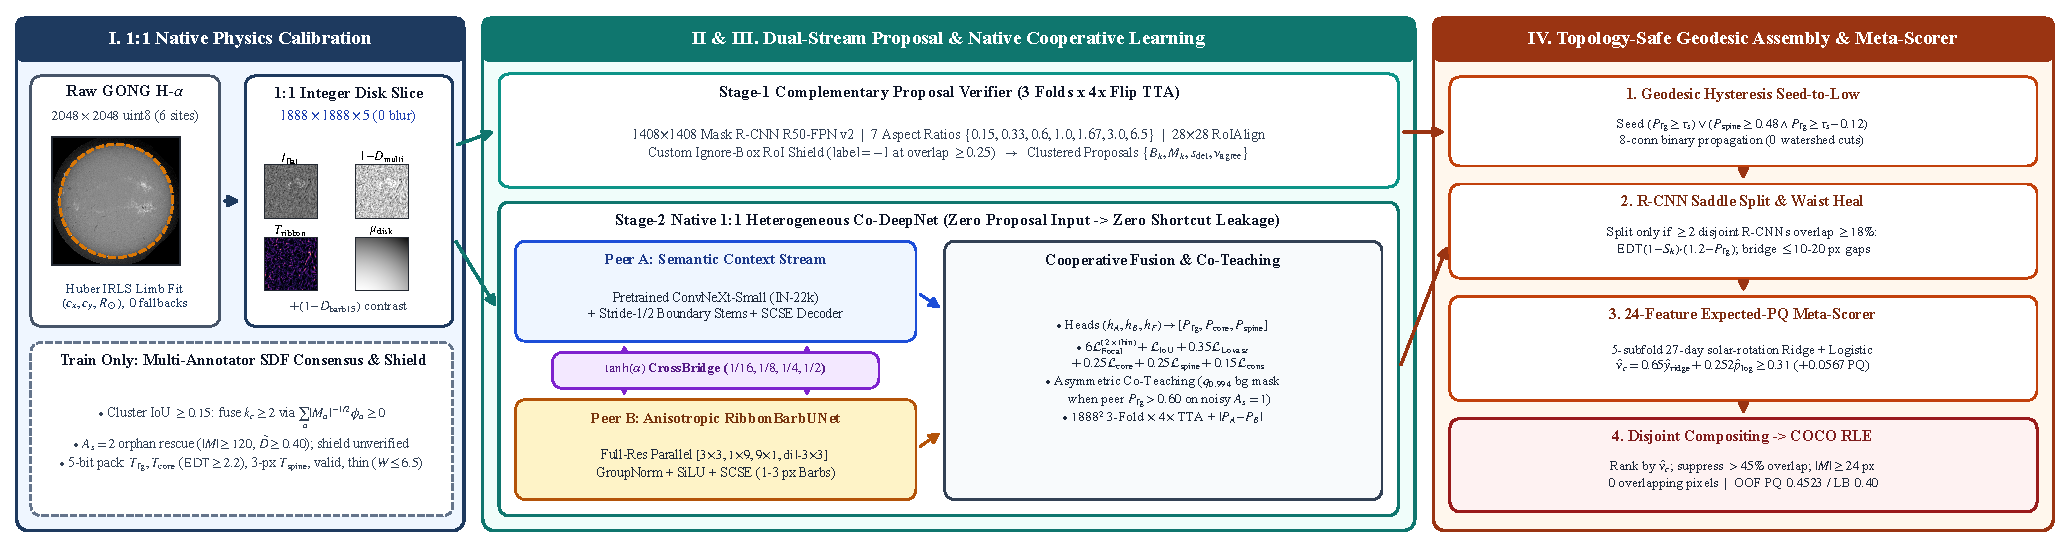
\includegraphics[width=\textwidth]{fig1_architecture_pipeline.pdf}
    \vspace{-8pt}
    \caption{Physics-guided cooperative framework: (I)~full-resolution $1888^2 \times 5$ chromospheric calibration and zero-bloat SDF consensus fusion, (II)~ignore-shielded $1408^2$ Mask R-CNN object verifier, (III)~decoupled heterogeneous cooperative streams (ConvNeXt-Small context peer + full-resolution anisotropic strip peer) with $\tanh(\alpha)$ cross-scale bridges and co-teaching, and (IV)~geodesic hysteresis, dual-detector Voronoi cuts, waist healing, and $24$-feature expected-PQ scoring.}
    \vspace{-6pt}
    \label{fig:architecture}
\end{figure*}

    Every stage of our framework follows from provable empirical bounds. Section~\ref{sec:oracles} derives resolution, topological-cut, and marginal-PQ multi-observer laws on slender ribbons. Section~\ref{sec:methodology} details our $1888 \times 1888$ chromospheric tensor, ignore-shielded Mask R-CNN verifier \cite{he2017mask}, and decoupled cooperative architecture pairing ConvNeXt-Small \cite{liu2022convnet} with an anisotropic strip U-Net \cite{ronneberger2015unet} under asymmetric co-teaching \cite{han2018coteaching,yu2019coteaching}. Section~\ref{sec:evaluation} evaluates geodesic assembly and expected-PQ scoring across $361$ out-of-fold disks, lifting three-fold PQ from $0.3956$ to $0.4523$ ($+0.1156$ above pairwise human agreement).

% ==================================== %
%     EMPIRICAL ORACLES & THEORY       %
% ==================================== %
\section{Empirical Bounds and Multi-Observer Theory}\label{sec:oracles}

\subsection{Resolution Loss and the Sub-Pixel Erosion Cliff}
    Before changing architectures, we passed all $6{,}982$ development masks ($981$ entries across $601$ disks) through the competition metric \cite{kirillov2019panoptic}. Skeleton Euclidean distance transforms (EDT) confirm extreme slenderness: median centerline length is $147.9$~px whereas median width $W = 2\,\text{median}(\text{EDT})$ is $8.25$~px, with $18.3\%$ of all instances having $W \le 6$~px. Downsampling ground-truth masks onto a $512 \times 512$ or $1024 \times 1024$ grid and bilinearly restoring them to $2048^2$ already forfeits $0.0801$ PQ ($90\%$ CI $[0.0780, 0.0823]$) and $0.0222$ PQ (Figure~\ref{fig:quant_oracles}(a)). Resolution loss is irreversible.

    Contour perturbations around $\text{IoU} > 0.50$ are sharply asymmetric, since uniform $1$-px dilation costs $0.1751$ PQ. Erosion hurts far worse. Shrinking contours by $1$~px loses $0.2149$ PQ, and a $2$-px erosion destroys $0.5156$ PQ by pushing $96.6\%$ of thin ribbons ($W \le 6$~px) below $\text{IoU} = 0.50$. Wide Gaussian blur augmentation ($\sigma_{\text{eff}} \approx 16.52$~px) similarly attenuated thin-ribbon contrast to $\operatorname{erf}(W / 2\sqrt{2}\sigma) = 11.5\%$, erasing $61.2\%$ of thin filaments while forcing surviving thin TPs to over-dilate ($+0.73$~px) and wide ribbons ($>24$~px) to erode inward ($-7.10$~px). Blur caused both errors. Capping blur at $\sigma_{\text{aug}} \le 1.25$~px at native pixel pitch eliminates both biases.

\subsection{Topological Cut Fragility on Branched Ribbons}
    To test whether watershed or boundary-cut heads suit coronal flux ropes, we evaluated exact foreground unions across all $601$ development disks. Plain $8$-connected components ($\ge 50$~px) recover $0.9989$ PQ against the $0.9998$ disjoint ceiling ($9$ merges across $6{,}982$ instances). Injecting a $30\%$ false transverse cut rate into an idealized $1$-px contact-band splitter collapses PQ to $0.8157$ and spawns $2{,}033$ fragments because one transverse cut severs a slender ribbon into two unmatched halves. Topology must stay intact. Global watershed is disabled, and components split only where two disjoint object detections verify a saddle.

\begin{figure*}[t]
    \centering
    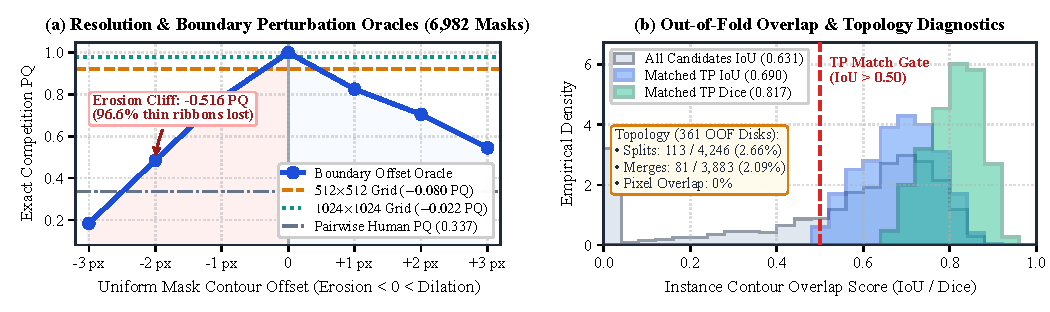
\includegraphics[width=\textwidth]{fig2_oracles_and_quant_diagnostics.pdf}
    \vspace{-8pt}
    \caption{Empirical bounds and out-of-fold overlap diagnostics. (a)~Exact competition PQ under uniform mask erosion/dilation and downsampled output grids ($6{,}982$ development masks) vs.\ pairwise human agreement ($0.337$). (b)~Empirical IoU and Dice distributions across $361$ out-of-fold disks ($2{,}687$ matched TPs and $3{,}883$ candidate comparisons) with topological split/merge rates.}
    \vspace{-6pt}
    \label{fig:quant_oracles}
\end{figure*}

\subsection{Multi-Observer Marginal-PQ Keep Calculus}
    MAGFiLO disks carry $A_s \in \{1, 2, 3\}$ independent human annotation entries ($411$, $145$, and $151$ training stems), all scored simultaneously against one deterministic prediction set. Scoring each observer against co-annotators across $598$ shared pairs yields a pairwise human PQ of $0.3367$ ($90\%$ CI $[0.3225, 0.3509]$, $\text{SQ}=0.6332$, $\text{RQ}=0.5317$, median union IoU $0.472$), split across boundary jitter ($29.4\%$), sub-threshold overlap ($29.4\%$), fibril omissions ($26.7\%$), and split/merge disputes ($14.5\%$).

    Under pooled multi-entry scoring, a candidate mask $C$ on a disk with $A_s$ entries improves $S_s / D_s$ whenever its expected marginal value clears zero:
\begin{equation}\label{eq:marginal_pq}
    v(C) = \frac{1}{A_s}\sum_{a=1}^{A_s} \mathbf{1}\!\left[\operatorname{IoU}(C, G_a^*) > 0.5\right]\!\left(\operatorname{IoU}(C, G_a^*) + \frac{1}{2}\right) - \frac{1}{2},
\end{equation}
    where $G_a^*$ is the best unmatched mask in entry $a$. Across $2{,}319$ clusters, single-observer orphans ($k_c = 1$) on $A_s = 3$ disks carry negative expected value ($v = -0.1667$), whereas $k_c \ge 2$ clusters are strictly positive ($+0.2492$ on $A_s=2$, $+0.1788$ on $A_s=3$). Single-observer orphans lose points. Because pixel unions bloat widths ($0.3273$ held-out human PQ), we fuse $k_c \ge 2$ cluster masks $\{M_m\}$ via an inverse-$\sqrt{\text{area}}$-weighted Signed Distance Field (SDF) zero-level set:
\begin{equation}\label{eq:sdf_fusion}
    \psi(\mathbf{x}) = \frac{\sum_{m \in \mathcal{C}} |M_m|^{-1/2}\!\left(\operatorname{EDT}(M_m)(\mathbf{x}) - \operatorname{EDT}(\neg M_m)(\mathbf{x})\right)}{\sum_{m \in \mathcal{C}} |M_m|^{-1/2}} \ge 0.
\end{equation}
    Level set $\psi(\mathbf{x}) \ge 0$ preserves geometric-mean ribbon width and lifts held-out human consensus PQ to $0.3850$. On $A_s = 2$ disks, dark orphans ($|M| \ge 120$~px, $\tilde{D}_{\text{multi}} \ge 0.40$) are kept, while unverified singletons form a dilated ignore shield.

% ==================================== %
%              METHODOLOGY             %
% ==================================== %
\section{Methodology}\label{sec:methodology}
    Figure~\ref{fig:architecture} outlines our four-stage system. Every prior, threshold, and meta-weight is fitted strictly out-of-fold.

\subsection{Stratified Split and 5-Channel Native Physics}
    We reserved a $15\%$ holdout split ($106$ untouched disks) prior to exploratory modeling and partitioned the $601$ development disks into five group-preserving folds ($[119,\allowbreak 121,\allowbreak 121,\allowbreak 121,\allowbreak 119]$ stems) balanced by station, solar-cycle phase, and $A_s$. Our final ensemble trains three fold models, validating out-of-fold on Folds~0--2 ($361$ disks, $4{,}246$ instances) from the $\approx 480$ complementary disks per fold.

    Raw $8$-bit GONG images exhibit limb darkening, plage rings, and gain drift across Big Bear (\texttt{Bh}), Cerro Tololo (\texttt{Ch}), Learmonth (\texttt{Lh}), Mauna Loa (\texttt{Mh}), Teide (\texttt{Th}), and Udaipur (\texttt{Uh}), yielding cross-site $\eta^2 = 0.1404$ and raw $\text{SNR} = 1.37$. Radial gradient scanning ($360$ azimuths, $r \in [860, 945]$~px) with four-step Huber IRLS ($\delta = 2.0$) fits $(c_x, c_y, R_\odot)$ across all $887$ frames ($R_\odot \in [892, 922]$~px, $0$ fallbacks). Since $2 R_\odot \le 1844 < 1888 = 59 \times 32$, a centered $1888 \times 1888$ integer crop captures $100\%$ of the disk at native pitch. Zero interpolation blur occurs.

    On a $512^2$ grid clamped outside $0.982 R_\odot$, we suppress plage via $\min(I, G_{18}(I) + 18)$, apply $21 \times 21$ elliptical closing, and smooth at $\sigma \in \{7, 20\}$ for quiet-Sun envelopes $(B_{\text{mid}}, B_{\text{broad}})$ and MAD noise $s_{\text{2D}}$ \cite{lindeberg1998edge}. Upsampling only smooth envelopes to $2048^2$ preserves crisp pixel texture across five GPU channels: flattened $I_{\text{flat}}$, inverted multi-scale absorption $1 - D_{\text{multi}}$, inverted $15 \times 15$ barb contrast $1 - D_{\text{barb15}}$, $\sigma^2$-normalized Hessian tubularity $T_{\text{ribbon}}$ ($\sigma \in \{1.2, 2.4, 4.8\}$) \cite{frangi1998multiscale}, and foreshortening $\mu_{\text{disk}} = \sqrt{\max(0, 1 - \rho^2)}$, cutting $\eta^2$ to $0.0878$ and raising SNR to $4.77$ ($\text{ROC-AUC} = 0.992$).

\subsection{Ignore-Shielded Object Proposal Verifier}
    Connected components cannot separate X-shaped saddles between touching flux ropes. Stage~II trains a $1408^2$ Mask R-CNN ResNet-50-FPN \cite{he2017mask} ($12$ epochs/fold, EMA $0.997$, $28 \times 28$ RoIAlign) with anchors $\{12,\allowbreak 24,\allowbreak 48,\allowbreak 96,\allowbreak 192\}$ and seven aspect ratios $\{0.15,\allowbreak 0.33,\allowbreak 0.6,\allowbreak 1.0,\allowbreak 1.67,\allowbreak 3.0,\allowbreak 6.5\}$. Our ignore-shield RoI sampler sets $\text{label} = -1$ whenever proposals overlap an unverified singleton box by $\ge 0.25$ of box area, avoiding false-negative suppression. Multi-fold $4\times$ flip TTA clusters masks at $\text{IoU} \ge 0.45$ to output $s_{\text{det}}$ and view agreement $v_{\text{agree}}$.

\begin{figure*}[t]
    \centering
    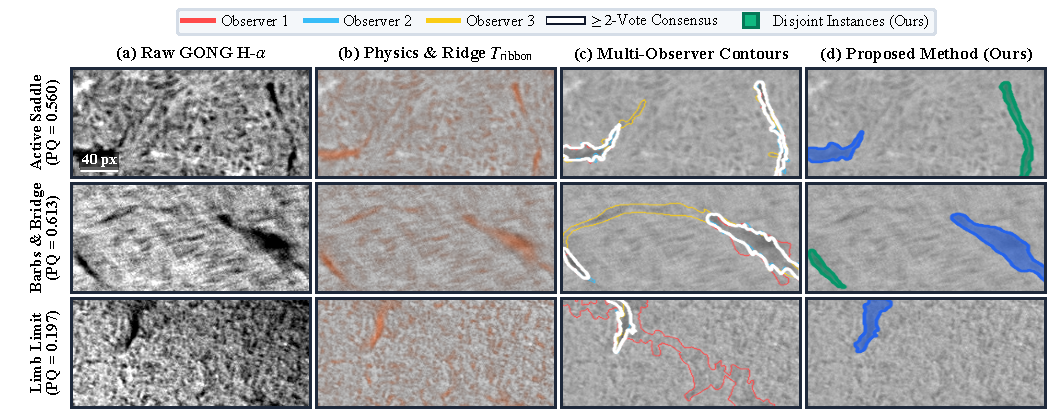
\includegraphics[width=\textwidth]{fig3_qualitative_barb_gallery.pdf}
    \vspace{-8pt}
    \caption{High-magnification full-resolution qualitative comparisons ($260 \times 134$~px out-of-fold crops): (a)~raw GONG H-$\alpha$, (b)~calibrated absorption blended with Hessian tubularity $T_{\text{ribbon}}$, (c)~human observers ($1$--$3$) and $\ge 2$-vote consensus (white), and (d)~our disjoint predictions across active-belt saddles (top), $1$--$2$~px barbs vs.\ spurious bridging (middle), and extreme-limb / orphan misses (bottom).}
    \vspace{-6pt}
    \label{fig:qualitative_gallery}
\end{figure*}

\subsection{Decoupled Heterogeneous Cooperative Network}
    Early two-stage prototypes ($0.4247$ PQ) cropped $256^2$ RoIs and fed proposal masks into the refiner, causing coarse mask shortcutting and clipped barbs (re-coupling lost $-0.0501$ PQ). Shortcut leakage vanished once dense segmentation dropped all proposal inputs.

    Our cooperative network pairs two heterogeneous peers at full resolution. The \textbf{Context Peer} adapts an ImageNet-22k ConvNeXt-Small encoder \cite{liu2022convnet} ($5$-channel stem) with stride-1/stride-2 boundary stems bypassing the $4 \times 4$ patchify bottleneck into an SCSE U-Net decoder \cite{roy2018scse}. The \textbf{Anisotropic Strip Peer} runs from stride-1 ($[32, 64, 128, 192, 256]$ channels) using parallel directional strip convolutions ($3 \times 3$, $1 \times 9$, $9 \times 1$, and dilated $3 \times 3$ with GroupNorm, SiLU, SCSE, and residual skips) to trace $1$--$3$~px barbs, linked via zero-initialized $\tanh(\alpha)$ cross-scale bridges at scales $1/16$--$1/2$.

    Heads $(h_A, h_B, h_F)$ predict foreground $P_{\text{fg}}$, core $P_{\text{core}}$ ($\text{EDT} \ge 2.2$~px), and $3$-px medial spine $P_{\text{spine}}$ ($20$ epochs/fold, $768^2$ crops, $70\%$ thin/\allowbreak near-limb oversampled, $D_4$ flips):
\begin{equation}\label{eq:coop_loss}
    \mathcal{L}_k = 6.0\,\mathcal{L}_{\text{Focal}}^{(2\times\text{thin})} + \mathcal{L}_{\text{SoftIoU}} + 0.35\,\mathcal{L}_{\text{Lov\'{a}sz}} + 0.25\,\mathcal{L}_{\text{core}} + 0.25\,\mathcal{L}_{\text{spine}},
\end{equation}
    doubling focal weight on $W \le 6.5$~px ribbons \cite{lin2017focal,berman2018lovasz} plus $0.15\,\|P_A - P_B\|_2^2$ consistency. Co-teaching filters label noise. From epoch~8, background pixels where one peer predicts $P_{\text{fg}} > 0.60$ above the $0.994$ focal-loss quantile are masked from its partner's gradient on noisy $A_s = 1$ disks. Full-disk $1888^2$ $4\times$ TTA (\texttt{fp16}) blends $0.50 P_F + 0.25 P_A + 0.25 P_B$ and $|P_A - P_B|$.

\subsection{Geodesic Assembly and Expected-PQ Scorer}
    Four deterministic steps follow. First, $8$-connected geodesic hysteresis grows seeds $(P_{\text{fg}} \ge \tau_s) \lor (P_{\text{spine}} \ge 0.48 \land P_{\text{fg}} \ge \tau_s - 0.12)$ down to $\tau_s - \Delta_{\text{hyst}}$. Splits require dual confirmation. Components ($\ge 140$~px) cut \emph{only} when $\ge 2$ disjoint ($\text{IoU} < 0.12$) proposal masks ($s_{\text{det}} \ge 0.44$) each cover $\ge 60$~px and $\ge 18\%$ of detection area via minimum $d_k(\mathbf{x}) = \operatorname{EDT}(\neg S_k)(\mathbf{x}) \cdot (1.20 - P_{\text{fg}}(\mathbf{x}))$. Third, waist healing bridges $20$-px gaps inside one proposal mask ($s_{\text{det}} \ge 0.42$, $\bar{P}_{\text{fg}} \ge 0.18$) or $10$-px collinear spine gaps ($\bar{P}_{\text{fg}} \ge 0.28, \bar{P}_{\text{spine}} \ge 0.22$) unless vetoed by disjoint boxes, and rescues uncovered detections ($s_{\text{det}} \ge 0.48$, $\ge 28$~px at $P_{\text{fg}} \ge 0.20$).

    Fourth, $24$ candidate features span probabilities ($P_{\text{fg}}$ mean/\allowbreak $q_{85}$/\allowbreak max, $P_{\text{core}}$, $P_{\text{spine}}$, $1 - \overline{|P_A - P_B|}$, perimeter drop), detector support ($s_{\text{det}}$, IoU, $v_{\text{agree}}$), physics ($D_{\text{multi}}$, $D_{\text{barb15}}$, $T_{\text{ribbon}}$ medians/$q_{90}$, SNR, edge contrast, outer plage $q_{95}$, $\mu_{\text{disk}}$), and shape ($\log(1+\text{area})$, fill, elongation, circularity). Ridge ($\alpha=40$) and $L_2$ Logistic ($\lambda=5$) models fit five $27$-day rotation subfolds to predict $y_c \in [0, 1]$:
\begin{equation}\label{eq:metascorer}
    \hat{v}_c = 0.65\,\operatorname{clip}(\tilde{\mathbf{x}}_c^\top \mathbf{w}_{\text{ridge}}, 0, 1) + 0.35 \cdot 0.72\,\sigma(\tilde{\mathbf{x}}_c^\top \mathbf{w}_{\text{log}}).
\end{equation}
    Candidates with $\hat{v}_c \ge 0.31$ and $|M_c| \ge 24$~px composite greedily onto a $2048^2$ ownership buffer, suppressing $>45\%$ overlap. Duplicate pixels never occur.

\begin{table}[b]
    \vspace{-6pt}
    \caption{Three-fold out-of-fold validation performance across folds, observer strata ($A_s$), and consensus targets ($90\%$ CIs).}
    \vspace{-8pt}
    \label{tab:oof_breakdown}
    \centering
    \resizebox{\columnwidth}{!}{%
    \begin{tabular}{lcccccc}
        \toprule
        \textbf{Validation Cohort} & \textbf{Disks} & \textbf{GT} & \textbf{PQ [90\% CI]} & \textbf{SQ} & \textbf{RQ} & \textbf{Split/Merge} \\
        \midrule
        Fold 0 (OOF) & 119 & 1,339 & 0.4473 [0.430, 0.464] & 0.6841 & 0.6539 & 47 / 24 \\
        Fold 1 (OOF) & 121 & 1,539 & 0.4374 [0.417, 0.457] & 0.6830 & 0.6404 & 44 / 30 \\
        Fold 2 (OOF) & 121 & 1,368 & 0.4731 [0.457, 0.489] & 0.6853 & 0.6903 & 22 / 27 \\
        \textbf{Pooled 3-Fold OOF} & \textbf{361} & \textbf{4,246} & \textbf{0.4523 [0.442, 0.463]} & \textbf{0.6841} & \textbf{0.6611} & \textbf{113 / 81} \\
        \midrule
        Single-Entry ($A_s=1$) & 205 & 1,613 & 0.4687 [0.455, 0.482] & 0.6896 & 0.6797 & 31 / 33 \\
        Dual-Entry ($A_s=2$) & 74 & 1,102 & 0.4522 [0.433, 0.472] & 0.6844 & 0.6608 & 32 / 19 \\
        Triple-Entry ($A_s=3$) & 82 & 1,531 & 0.4366 [0.416, 0.457] & 0.6784 & 0.6436 & 50 / 29 \\
        Zero-Bloat SDF Consensus & 361 & 3,081 & 0.4959 [0.484, 0.507] & 0.7061 & 0.7023 & 68 / 54 \\
        \textbf{Multi-Observer ($\ge 2$ Votes)} & \textbf{156} & \textbf{1,492} & \textbf{0.5363 [0.521, 0.551]} & \textbf{0.7294} & \textbf{0.7353} & \textbf{29 / 21} \\
        \bottomrule
    \end{tabular}%
    }
\end{table}

% ==================================== %
%              EVALUATION              %
% ==================================== %
\section{Evaluation}\label{sec:evaluation}

\subsection{Evaluation Strategy and Uncertainty Protocol}
    Submissions are ranked by pooled Panoptic Quality \cite{kirillov2019panoptic} accumulated across all validation entries before division:
\begin{equation}\label{eq:pq_def}
    \text{PQ} = \underbrace{\frac{\sum_{(p,g) \in \text{TP}} \operatorname{IoU}(p,g)}{|\text{TP}|}}_{\text{Segmentation Quality (SQ)}} \times \underbrace{\frac{|\text{TP}|}{|\text{TP}| + \frac{1}{2}|\text{FP}| + \frac{1}{2}|\text{FN}|}}_{\text{Recognition Quality (RQ)}},
\end{equation}
    matched greedily at $\operatorname{IoU}(p,g) > 0.50$. For $27$-day rotational autocorrelation ($\hat{\rho}_u = +0.32$ at $1$--$3$~d lag), we run $2{,}000$-replicate bootstrap $90\%$ CIs over stems and rotation blocks ($1$--$54$~d), requiring $+0.0030$ PQ lift.

\begin{table}[b]
    \vspace{-6pt}
    \caption{Progressive architecture study and controlled negative ablations on Fold~0 ($119$ disks).}
    \vspace{-8pt}
    \label{tab:ablations}
    \centering
    \scriptsize
    \setlength{\tabcolsep}{2.8pt}
    \begin{tabularx}{\columnwidth}{Xccc}
        \toprule
        \textbf{Method / Controlled Ablation} & \textbf{Fold-0 PQ} & \textbf{$\Delta$ PQ} & \textbf{LB} \\
        \midrule
        Inter-Observer Pairwise Baseline ($598$ pairs) & 0.3367 & -- & -- \\
        ResUNet-34 Baseline (Raw H-$\alpha$, $\sigma{=}16.5$ blur) & 0.3332 & -- & -- \\
        $+$ 5-Ch Chromospheric Physics \& Medial Spine & 0.3714 & $+0.0382$ & -- \\
        $+$ Mask R-CNN \& Coupled $256^2$ RoI Refiner & 0.4247 & $+0.0533$ & -- \\
        $+$ Decoupled Full-Res Cooperative Net (1-Fold) & 0.4457 & $+0.0210$ & 0.39 \\
        \midrule
        w/ Global 5-Level Optical-Depth Max-Tree & 0.3911 & $-0.0546$ & -- \\
        w/ Coupled Proposal Mask Input (RoI Shortcut) & 0.3956 & $-0.0501$ & -- \\
        w/ Heuristic Scoring Only (No Meta-Scorer) & 0.3956 & $-0.0517$ & -- \\
        w/ Inverse-Area Instance-Equalized Loss & 0.4312 & $-0.0145$ & -- \\
        w/ Unclamped Background Envelope & 0.4338 & $-0.0119$ & -- \\
        \midrule
        \textbf{Proposed Full Cooperative Framework} & \textbf{0.4473} & \textbf{$+0.1141^\dagger$} & \textbf{0.40}$^\ddagger$ \\
        \bottomrule
    \end{tabularx}
    \vspace{1pt}
    {\raggedright\scriptsize $^\dagger$Gain over ResUNet-34 baseline. $^\ddagger$Three-fold ensemble ($0.4523$ OOF PQ, $1{,}183$ disjoint test instances across $177/180$ disks in $53.8$~min offline on NVIDIA T4).\par}
\end{table}

\subsection{Quantitative Distributions and Ablations}
    Table~\ref{tab:oof_breakdown} and Figure~\ref{fig:quant_oracles}(b) summarize three-fold OOF metrics across $361$ disks ($599$ entries). Pooled PQ reaches $0.4523$ ($90\%$ CI $[0.4418,\allowbreak 0.4627]$, $\text{SQ}=0.6841$, $\text{RQ}=0.6611$, $2{,}687$ TPs, $1{,}196$ FPs, $1{,}559$ FNs), peaking at $0.4731$ on Fold~2 and scoring $0.40$ on the Kaggle Public Leaderboard ($+0.01$ over single-fold). Raw PQ drops from $0.4687$ ($A_s = 1$) to $0.4366$ ($A_s = 3$) purely from inter-observer denominator conflicts, whereas SDF consensus and $\ge 2$-vote scoring ($156$ disks) reach $0.4959$ and $0.5363$ PQ ($\text{SQ}=0.7294$, $\text{RQ}=0.7353$).

    Contour adherence stays tight. Across $2{,}687$ matched TPs in Figure~\ref{fig:quant_oracles}(b), IoU averages $0.6841 \pm 0.0848$ (median $0.6901$, IQR $[0.6214,\allowbreak 0.7495]$) and Dice averages $0.8094 \pm 0.0607$ (median $0.8166$, IQR $[0.7665,\allowbreak 0.8568]$), while all $3{,}883$ candidate comparisons hit median IoU $0.6312$ (Dice $0.7739$, $69.2\% > 0.50$). Splits affect $113/\allowbreak 4{,}246$ ribbons ($2.66\%$: $100$ two-way, $12$ three-way, $1$ four-way) and merges affect $81/\allowbreak 3{,}883$ predictions ($2.09\%$: $78$ two-way, $3$ three-way). Expected-PQ scoring adds $+0.0567$ OOF PQ ($0.3956 \to 0.4523$ at $\tau_s \in \{0.54,\allowbreak 0.58\}$, $\hat{v}_c \ge 0.31$). Top weights favor $s_{\text{det}}$ ($+0.114$), mean $P_{\text{fg}}$ ($+0.113$), and peer agreement ($+0.106$) while penalizing $\max(P_{\text{fg}})$ ($-0.098$) on sunspots.

    Table~\ref{tab:ablations} isolates each stage: chromospheric physics and spine heads cut FPs by $53\%$ ($+0.0382$ PQ), object proposals added $+0.0533$, and full-resolution decoupling added $+0.0210$. Negative ablations confirmed why. Optical-depth max-trees ($-0.0546$), coupled RoI mask inputs ($-0.0501$), and inverse-area weights ($-0.0145$) failed by violating our cut-fragility, barb-clipping, and orphan-utility bounds.

\subsection{Qualitative Forensics and Limitations}
    Figure~\ref{fig:qualitative_gallery} inspects pixel-scale masks: Row~1 (\texttt{2014\allowbreak 0205\allowbreak 180154Bh}) separates colinear active-belt ribbons across a saddle while keeping $1$--$2$~px barbs, and Row~2 (\texttt{2012\allowbreak 0715\allowbreak 123434Ch}, $\text{PQ}=0.613$) rejects a $90$-px observer bridge (yellow) in favor of $\ge 2$-vote cores. Limb foreshortening stays hard. Near $\rho > 0.95$ ($\mu_{\text{disk}} < 0.31$, Row~3 \texttt{2012\allowbreak 0703\allowbreak 070814Th}, $\text{PQ}=0.197$), $2$-px slivers mimic spicules ($0.000$ PQ on $14$ solar-minimum frames), and single-observer channels (red) cap RQ, motivating $\pm 6$~h rotation warping and GONG $B_\parallel$ magnetogram fusion.

\clearpage
% ==================================== %
%            ACKNOWLEDGMENT            %
% ==================================== %
\section{Acknowledgment}\label{sec:acknowledgment}
    % Do not change
    The organization of the Filament Segmentation Challenge 2026 is partially supported by the U.S. National Science Foundation (NSF) under Grant No. 2209912 and 2433781, directorate for Computer and Information Science and Engineering (CSE), and Office of Advanced Cyberinfrastructure (OAC), and Grant No. 2511630, AST Division Of Astronomical Sciences and MPS Directorate for Mathematical and Physical Sciences.

    The Filament Segmentation Challenge 2026 is sponsored by the U.S. National Science Foundation (NSF) National Solar Observatory (NSO). 

    This work utilizes GONG data obtained by the NSO Integrated Synoptic Program, managed by the National Solar Observatory, which is operated by the Association of Universities for Research in Astronomy (AURA), Inc. under a cooperative agreement with the National Science Foundation and with contribution from the National Oceanic and Atmospheric Administration. The GONG network of instruments is hosted by the Big Bear Solar Observatory, High Altitude Observatory, Learmonth Solar Observatory, Udaipur Solar Observatory, Instituto de Astrofísica de Canarias, and Cerro Tololo Interamerican Observatory.

\bibliographystyle{ACM-Reference-Format}
\bibliography{main}

\end{document}
